\documentclass[12pt,a4paper]{article}
\usepackage{amsmath,amssymb,cite}
\usepackage{caption}
\usepackage{subcaption}
\usepackage{graphicx}
\usepackage{hyperref}
\usepackage{cite}

\usepackage[margin=0.75in]{geometry}

\usepackage{suffix}
\usepackage{mathtools}

\DeclarePairedDelimiterX\MeijerM[3]{\lparen}{\rparen}%
{\begin{smallmatrix}#1 \\ #2\end{smallmatrix}\delimsize\vert\,#3}

\newcommand\MeijerG[8][]{%
  G^{\,#2,#3}_{#4,#5}\MeijerM[#1]{#6}{#7}{#8}}

\WithSuffix\newcommand\MeijerG*[7]{%
  G^{\,#1,#2}_{#3,#4}\MeijerM*{#5}{#6}{#7}}
  
\newcommand{\brac}[1] {\!\left(#1\right)}

\newcommand{\rsb}{r_{sb}}

\begin{document}
We start with the \emph{Cornell + String Breaking} potential that is often employed in phenomenological studies,
\begin{equation}
\label{eq:VvacPheno}
V^{vac}\brac{r}=\begin{cases}
    \sigma r -\frac{\tilde{\alpha}_s}{r}; & r<r_{sb},\\
    \sigma r_{sb}-\frac{\tilde{\alpha}_s}{r}; &r\geq r_{sb},
  \end{cases}
\end{equation}
where \(r_{sb}\simeq 1.1\)GeV is the string-breaking radius. Following Thakur, Kakade, and Patra \cite{Thakur:2013nia}, we want to transform this into Fourier space, multiply by the in-medium complex permittivity and then transform back to real space. In Fourier transforming Eq.~\eqref{eq:VvacPheno}, the angular parts can be carried out as usual and the radial integration must be split into two regions \(\left[0,r_{sb}\right]\) and \(\left[r_{sb},\infty\right]\). The second of these must be regulated in a suitable manner to ensure convergence; as in \cite{Thakur:2013nia} we damp the integrand with an exponential factor \(e^{-ar}\) before taking the limit \(a\to 0\). The result for the string part of the potential is
\begin{equation}
\label{eq:VvacPhenoFourier}
V^{vac}_{S}\brac{p}=4\pi\sigma\rsb\Bigg(\frac{-2+\brac{2-p^2r_{sb}^2}\cos\brac{p r_{sb}}+2 p r_{sb}\sin\brac{p r_{sb}}}{\rsb\;p^4}+\frac{p r_{sb}\cos\brac{p r_{sb}}-\sin\brac{p r_{sb}}}{p^3}\Bigg).
\end{equation}
The medium modifications are accounted for by multiplying by the complex permittivity as follows:
\begin{equation}
\label{eq:VMedMod}
V_{S}\brac{r}=\int\frac{\mathrm{d}^3p}{\brac{2\pi}^3}V^{vac}_{S}\brac{p}\varepsilon^{-1}\brac{\mathbf{p},m_D}e^{i\mathbf{pr}},
\end{equation}
where
\begin{equation}
\label{eq:MedPerm}
\varepsilon^{-1}\!\left(\mathbf{p},m_{D}\right)=\frac{p^2}{p^2+m_D^2}-i\pi T \frac{p m_D^2}{\left(p^2+m_D^2\right)^2}.
\end{equation}
For the real part, this integration can be performed analytically, giving:
\begin{equation}
\label{eq:ReVs}
\mathrm{Re}V_{S}\brac{r}=\begin{dcases}
	\frac{\sigma e^{-m_D r}}{m_D^2r}[2+e^{m_D r}(-2+e^{-m_D\rsb}\brac{2+m_D\rsb}\sinh\brac{m_Dr})]+\mathrm{Re}\,c_S; & r<r_{sb},\\
    \frac{\sigma e^{-m_D r}}{{m_D^2r}}\left[2-2\cosh\brac{m_D\rsb}+m_D\rsb\sinh\brac{m_Dr}\right]+\mathrm{Re}\,c_S; &r\geq r_{sb},
  \end{dcases}
\end{equation}
where \(\mathrm{Re}\,c_S\) is chosen to ensure \(\mathrm{Re}V_{S}\brac{r\to 0}=0\) and \(\lim_{m_D\to0}\mathrm{Re}V_{S}\brac{r}=\sigma r\), namely
\begin{equation}
\mathrm{Re}\,c_S=\sigma\rsb-\frac{e^{-m_D\rsb}}{mD}\left[2+m_D\rsb+\sigma e^{m_D\rsb}\brac{m_D\rsb-2}\right].
\end{equation}
For the imaginary part, Eq.~\eqref{eq:VMedMod} can not be calculated analytically. However the angular integrations are performed to give the `most-analytical' form:
\begin{equation}
\label{eq:ImVs}
\mathrm{Im}V_{S}\brac{r}=-\frac{2\sigma}{\pi}\int_{0}^{\infty}\mathrm{d}p\;p^2\frac{\sin\brac{pr}}{pr}V^{vac}_{S}\brac{p}\mathrm{Im}\;\varepsilon^{-1}\brac{p,m_D}+\mathrm{Im}\,c_S,
\end{equation}
where again the constant term is chosen to ensure \(\mathrm{Im}V_{S}\brac{r\to 0}=0\):
\begin{equation}
\mathrm{Im}\,c_S=\frac{2\sigma}{\pi}\int_{0}^{\infty}\mathrm{d}p\;p^2V^{vac}_{S}\brac{p}\mathrm{Im}\;\varepsilon^{-1}\brac{p,m_D}.
\end{equation}
Eq.~\eqref{eq:ImVs} is straightforward to evaluate numerically.

After performing the Debye-mass fitting, the real part is able to reproduce the lattice data and the imaginary part flattens to a constant as required. See Figures.
\begin{figure}[h]
	\centering
	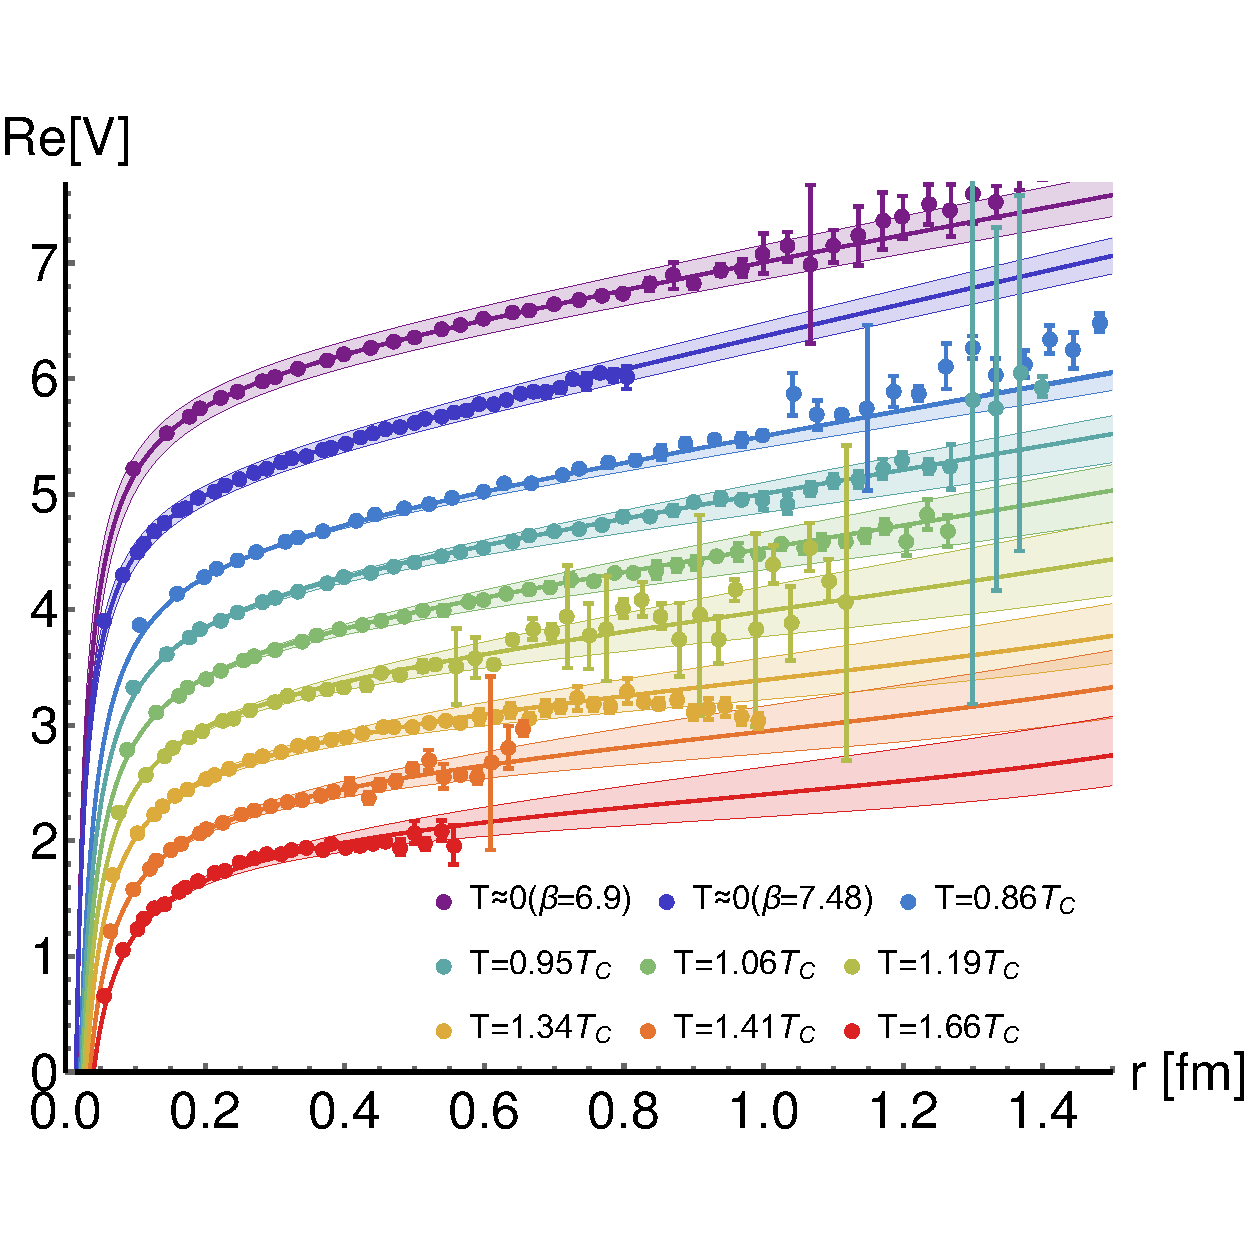
\includegraphics[width=11cm]{Debye_fitting} 
	\caption{Fitting of the real part.}    	
	\label{fig:ReVfit}
\end{figure}
\begin{figure}[h]
	\centering
	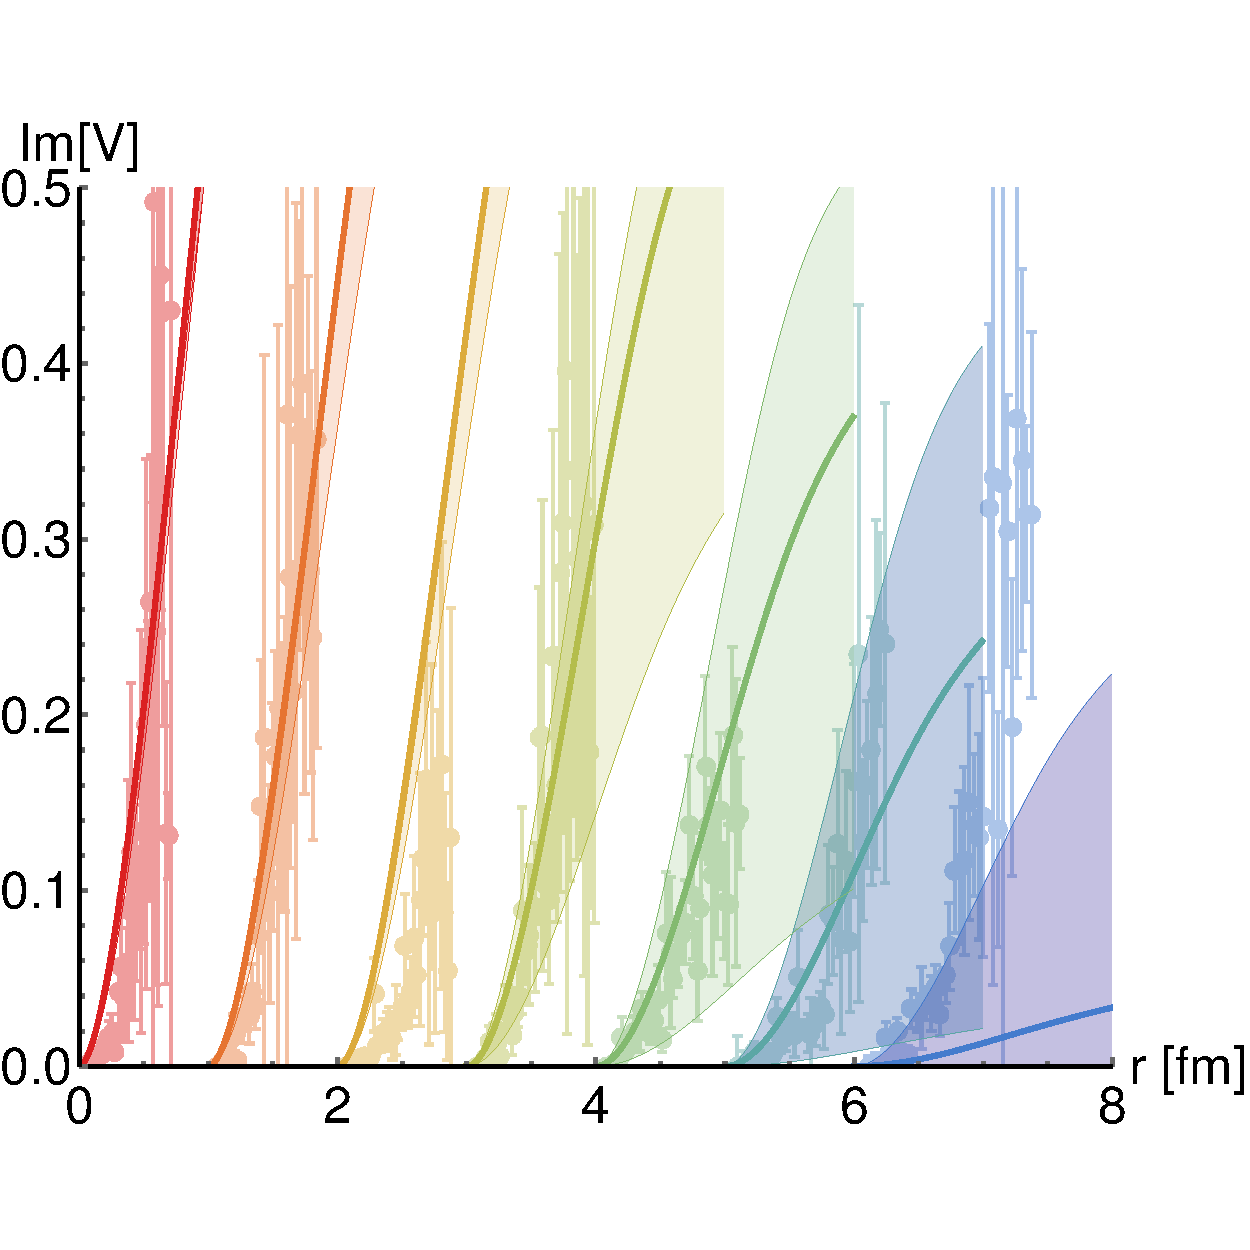
\includegraphics[width=11cm]{Debye_fitting2} 
	\caption{Resulting imaginary part.}    	
	\label{fig:ImVfit}
\end{figure}
\begin{figure}[h]
	\centering
	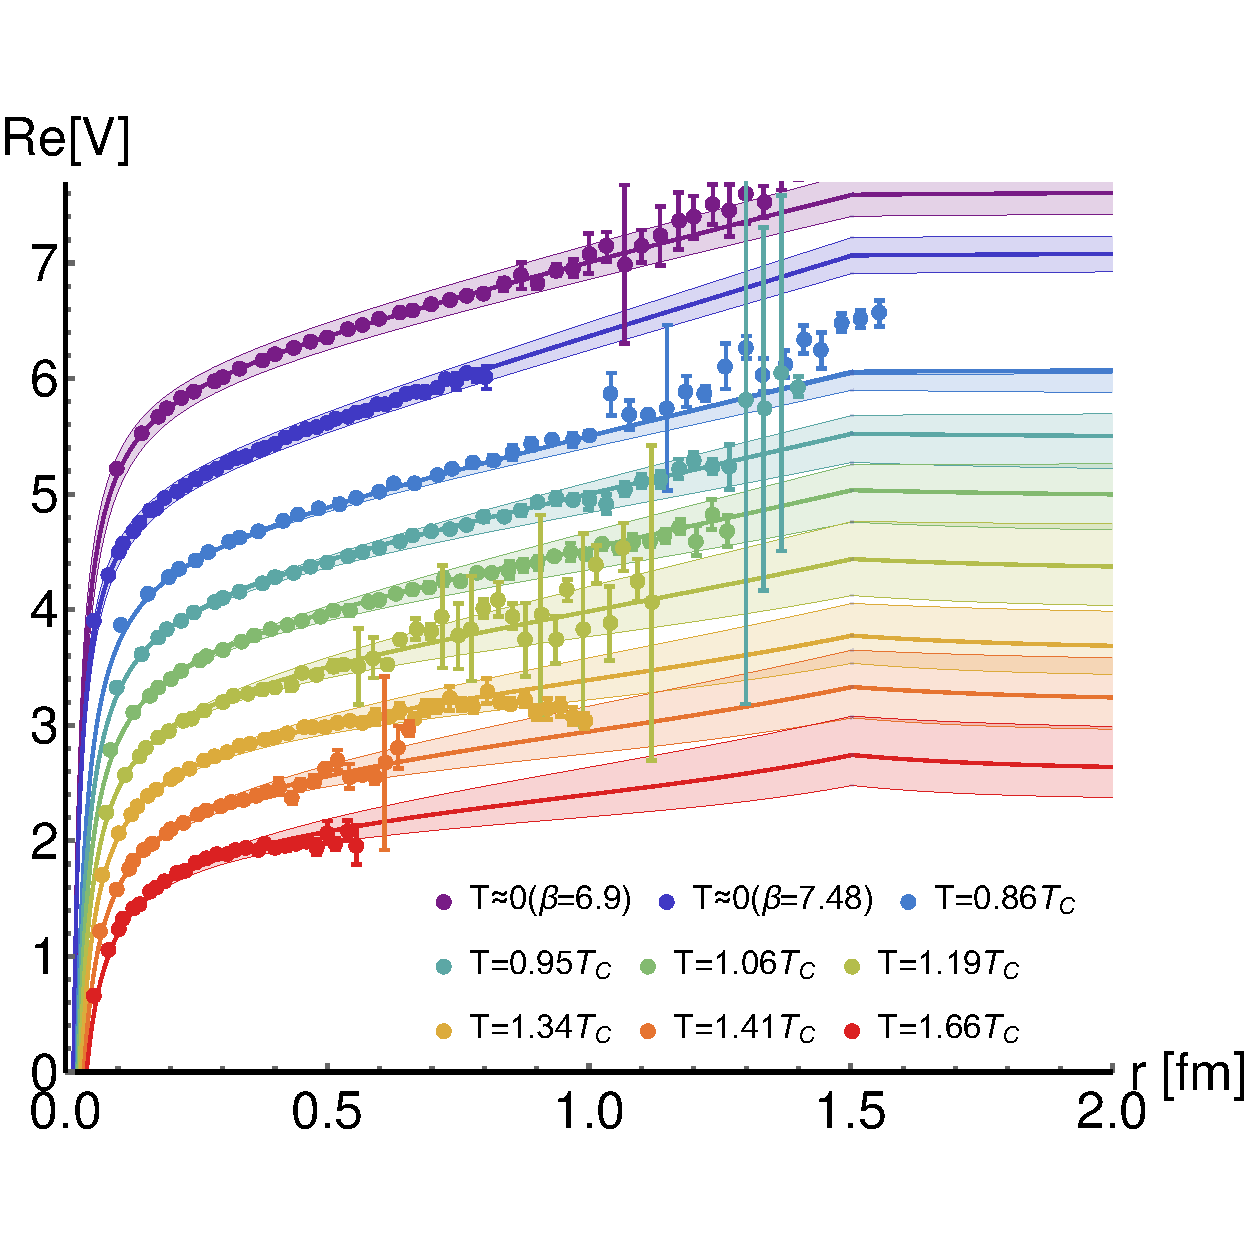
\includegraphics[width=11cm]{Debye_fitting3} 
	\caption{The real part contains a jump in the first derivative when \(r=\rsb\). For \(r>\rsb\) it quickly asymptotes to a constant.}    	
	\label{fig:ReVfit}
\end{figure}
\begin{figure}[h]
	\centering
	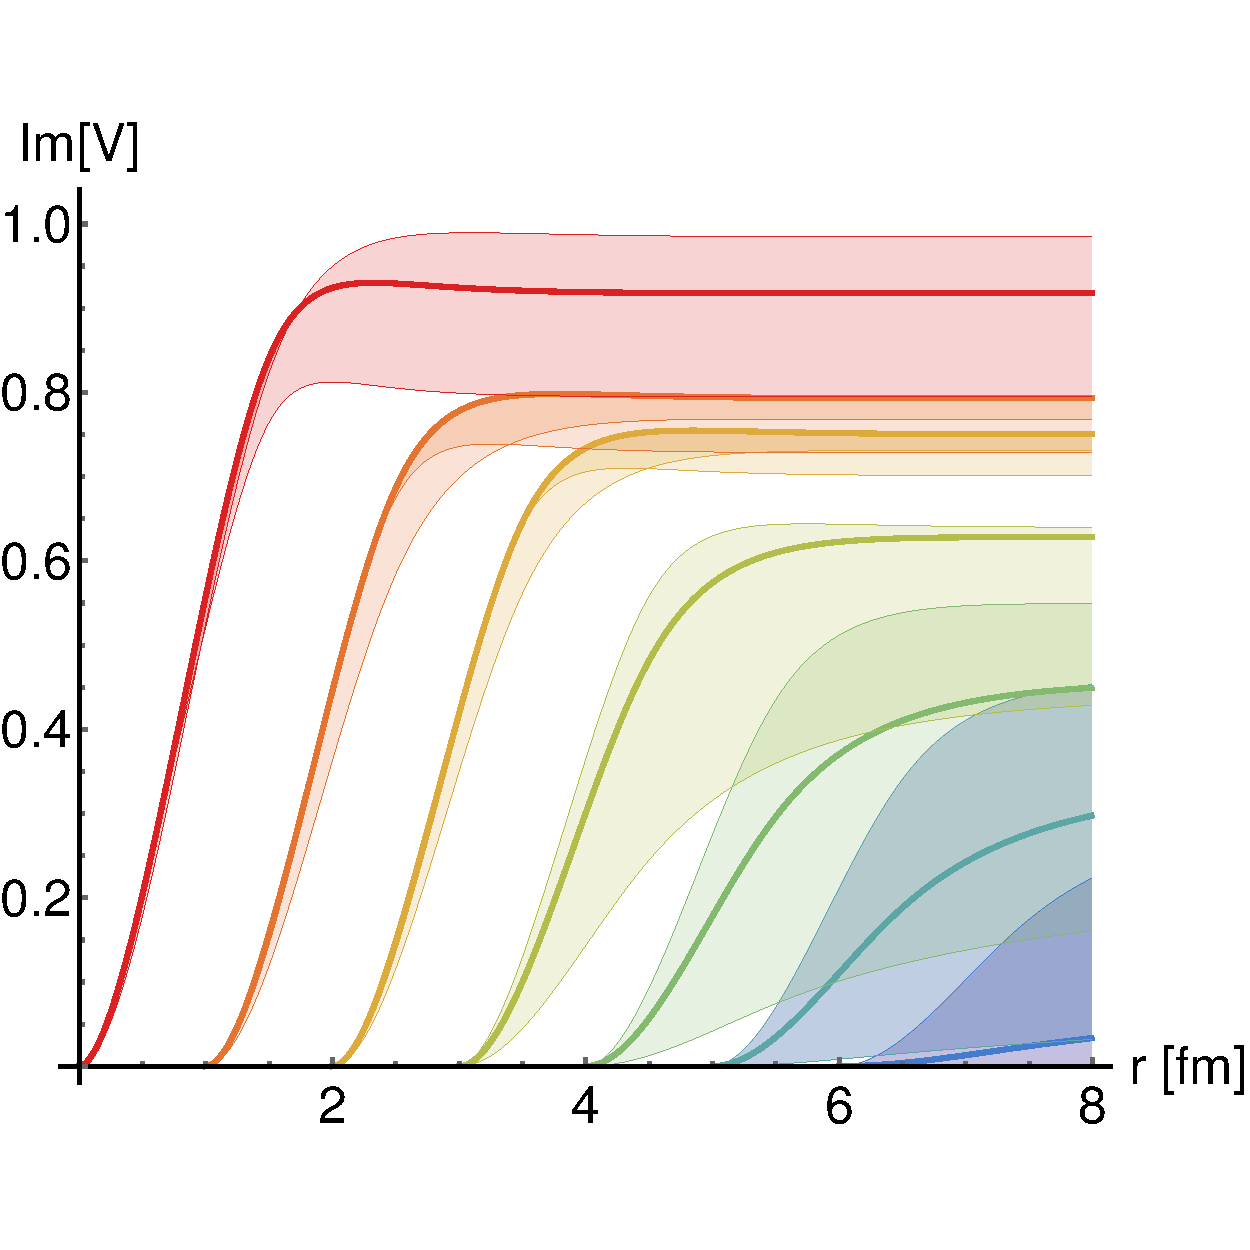
\includegraphics[width=11cm]{Debye_fitting1} 
	\caption{The imaginary part flattens off as required.}    	
	\label{fig:ImVfit}
\end{figure}

\bibliographystyle{plain}
\bibliography{pot_new1}

\end{document}